\documentclass{article}

\usepackage{multirow}
\usepackage{arxiv}
\usepackage{amsmath}

\usepackage[utf8]{inputenc} % allow utf-8 input
\usepackage[T1]{fontenc}    % use 8-bit T1 fonts
\usepackage{hyperref}       % hyperlinks
\usepackage{url}            % simple URL typesetting
\usepackage{booktabs}       % professional-quality tables
\usepackage{amsfonts}       % blackboard math symbols
\usepackage{nicefrac}       % compact symbols for 1/2, etc.
\usepackage{microtype}      % microtypography
\usepackage{lipsum}		% Can be removed after putting your text content
\usepackage{graphicx}
\usepackage{doi}
\usepackage{gensymb}


\title{Carbon Renaissance Whitepaper 1.0}

\author{

 \href{https://orcid.org/0000-0000-0000-0000}{
\includegraphics[scale=0.06]{orcid.pdf}\hspace{1mm}Greg Darragh}\\
	Carbon Renaissance\\
	\texttt{greg@crc.eco} \\
\And	
 \href{https://orcid.org/0000-0000-0000-0000}{
\includegraphics[scale=0.06]{orcid.pdf}\hspace{1mm}Mick Viner-Smith}\\
	Carbon Renaissance\\
	\texttt{mick@crc.eco} \\	
\And
 \href{https://orcid.org/0000-0000-0000-0000}{
\includegraphics[scale=0.06]{orcid.pdf}\hspace{1mm}Ian C. Moore, PhD}\\
	Syscoin Researcher\\
	\texttt{imoore@syscoin.org} \\
	\And
	\href{https://orcid.org/0000-0000-0000-0000}{
\includegraphics[scale=0.06]{orcid.pdf}\hspace{1mm}Jagdeep Sidhu, MSc} \\
	Syscoin Core Developer\\
	Blockchain Foundry Inc.\\
	\texttt{jsidhu@blockchainfoundry.co} \\
}

\renewcommand{\shorttitle}{Carbon Renaissance}

\hypersetup{
pdftitle={Stochastic Properties of EIP-1559 Basefees},
pdfsubject={q-bio.NC, q-bio.QM},
pdfauthor={Ian C. Moore, Jagdeep Sidhu},
pdfkeywords={Carbon Sequestration, Carbon Offsetting, Social Credit, NFT},
}

\begin{document}
\maketitle

\begin{abstract}

We introduce a carbon offsetting program through the tokenization of work done (ie, via Green tokens) on a blockchain. We utilize Non-fungible tokens as IOU contracts to facilitate engagement between stakeholders interested in pollution prevention and those performing the carbon offsetting. To incentivize adoption, a Black reward token is offered for those who utilize the system, which can be staked to acquire  Green tokens introduced to the supply

\end{abstract}

\keywords{Carbon Sequestration \and Carbon Offsetting  \and Social Credit \and NFT}

\section{Executive Summary}

\subsection{Mission and Vision}

We propose a Carbon offset design that creates natural economic incentives through business
processes on the blockchain tied to Non-fungible tokens (NFT) tokens issued from enterprise to participating companies which connect to Carbon offsetting processes. Upon audits of work, a fungible token (ie, Green token) is issued to companies involved based on a pre-negotiated ratio of tokens dispersed based on the quality of the work and quality of the credit-worthiness of the companies involved. Green tokens
represents auditing work done for carbon offsetting.

We conjecture that this will not only allow for incentives to modify spending behaviour of
consumers, but also produce a mechanism for stakeholders to adhere to carbon quotas by
purchasing and offsetting their carbon consumption through a novel token model. Furthermore, once our model is implemented for fair exchange of carbon tokens in auditable and censorship resistance mediums, we assert how this model can used to serve as a social credit component to a broader Universal Basic Income (UBI) model.

\subsection{Background}

Climate change is a well studied issue and is defined as global warming stemming from greenhouse gas emissions resulting from major shifts in weather patterns. As a result, it has recently garnered much attention on the world stage \cite{Kal96,Ten00,Hij05}. According to \cite{Glo21}, it is estimated that human activity accounts for 1.0 $^\circ$C of global warming above pre-industrial levels, and estimate that global warming is likely to reach 1.5$^\circ$C between 2030 and 2052. The EDGAR time series set shows that since the beginning of the 21$^{st}$ \cite{EDGAR19}, fossil CO$_{2}$ emissions have increased compared to the three previous decades; see Fig \ref{fig:edgars_co2_emissions}. It also shows that, as of 2018, global fossil CO$_{2}$ emissions have reached a total of 37.9 Gt CO$_{2}$. However, according to \cite{Liu20}, emissions have fallen \~ 1,900 MtCO$_{2}$ from 2019 to 2020 due mainly to the aviation and shipping sector due to the slowing of economic activity stemming from the 2020 pandemic. To combat this, carbon offsetting is the process by which many players are handling this issue. 

\begin{figure}[h]
\centering
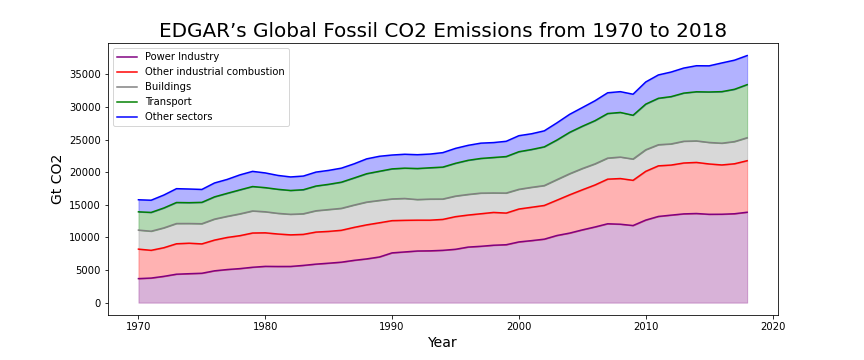
\includegraphics[width=5in]{edgars_co2_emissions.png}
\caption{Global Greenhouse Gas (GHG) emission per sector; see \cite{EDGAR19}. We can see the Power industry account for a large portion of global emissions, which provides insight as to where the largest opportunity for carbon reduction may be found.} 
\label{fig:edgars_co2_emissions}
\end{figure} 

Carbon offsetting is done via sequestration which is the process where atmospheric carbon dioxide is captured and stored for the purpose of abating climate change. After carbon is captured, it goes mainly one of two ways: (a) permanently stored underground; or (b) converted into a carbon-containing product \cite{CBC19}. Currently, the market for corporate procurement for carbon removal is very undeveloped. However, there are a number of organizations that have made strides to address this issue; which include Amazon, Apple, BCG, Delta, Facebook, Google, Mars, Shopify, Stripe, Swiss Re, United and Velux \cite{Mic21}. Of the aforementioned, Shopify, Stripe and Microsoft are making carbon removal a core focus in their business. More specifically Microsoft has a plan to remove carbon that they emit, and came to key conclusions. Namely, they can not meet current carbon negative commitments and estimate that they need to remove 6 Million Tons of carbon in 2030. Hence, an RFP was sent out in 2020 and 79 applications were received and 15 organizations were selected representing 1.3 Million metric tons of carbon removal. Their project selection process was based on several criteria: (a) Global carbon removal potential; (b) Affordability targeting \$15 per mtCO$_{2}$; (c) climate equity; (d) technology innovation; and (e) other sustainability dimensions. 

In 2019, the National Academies of Sciences, Engineering, and Medicine investigated the likely market size for Negative Emissions Technologies (NET), where they discuss how much carbon uptake is needed to meet Paris Agreement goals \cite{NET19}. They estimate that $\sim$ 10 GtCO$_{2}$ / yr is required globally by midcentury and $\sim$ 20 GtCO$_{2}$ / yr globally by centuries end to meet these goals. Six key sequestration technologies are identified which are: (a) coastal carbon blue; (b) terrestrial carbon removal and sequestration; (c) bioenergy with carbon capture and sequestration (BECCS); (d) geological sequestration; (e) direct air capture;  and (f) carbon mineralization. Of these aforementioned technologies, the former four are ready for large-scale deployment; see Table \ref{table:net} for estimated potential rates across US and the Globe.

\begin{table}[h]
\centering
\begin{tabular}{ |c|c|c|c| } 
\hline
 Negative Emission Technology & Estimated Cost (\$/tCo$_{2}$) &\multicolumn{2}{ c |}{ Upper Bound for Safe Potential rate of CO$_{2}$ (GtCO$_{2}$/y)}  \\
  & & US & Global \\
\hline
Coastal blue carbon & L & 0.02 & 0.13  \\
Afforestation / Reforestation & L & 0.15 & 1  \\
Forest management & L & 0.1 & 1.5  \\
Agricultural soils & L to M & 0.25 & 3  \\
BECCS & M & 0.5 & 3.5-5.2  \\
Direct air capture & H & 0 & 0  \\
Carbon mineralization & M to H & unknown & unknown \\
Total &  & 1.02 & 9.13-10.83 \\
\hline
\end{tabular}
\caption{Estimated potential rates of CO$_{2}$ removal for various Negative Emission Technologies (measured in GtCO$_{2}$ / y) for the US and across the globe (see \cite{NET19} for source), we see BECCS offer the best opportunity.}
\label{table:net}
\end{table}

\subsection{Problem Statement and Strategy}

We propose that token supply creation requires work, which include Carbon sequestration followed by an auditing process working with various stakeholders that are involved in the process. The minting of new token supply can be compared to Bitcoin's Proof-of-Work (PoW) process popularily described an \emph{mining}, which is a completely automated and trustless process. However, the Carbon Renaissance (CR) token minting process will be governed by a regulatory work-flow process working through various stakeholders, which will be covered throughout this whitepaper. Many of the market dynamics that we know which drive price discovery via the Bitcoin miner network can be utilized to understand the market dynamics with this project. Such dynamics include: (a) geographical advantages characteristic to the local environment; (b) regulations particular to certain jurisdictions that allow for more cost effective sequestration; and (c) technological advancements.

The token supply can work in both a inflation/deflation environment depending on the system setup. Whereas other projects are either strictly deflationary or inflationary. For instance, we show via simulation that it is possible to have the supply reach a state of equilibrium where supply is constant.  This economic feature can make it attractive for large corporate organizations and governments to work with.

The CR process works in a cycle where the token can move to one of three different states over time (ie, statetokens). These states are: (a) Green; (b) Red; and (c) Black, and are usecase dependant. Green tokens (ie,  otherwise refereed as base tokens) are purchased on exchanges and represent the potential of what can be utilized for carbon sequestration and are required to enter into the auditing process. Red tokens are non-tradable Non-Fungible Tokens (NFT) and represent unique IOU contracts between stakeholders who have intentions to sequester Carbon and those who offer the carbon sequestration service; see Fig. \ref{fig:red_to_green}. NFTs are unique digital assets that are stored on a blockchain and cannot be exchanged for one another, hence non-fungible. Finally, Black tokens represent sequestered carbon. For instance, 100 Black tokens represent proof of 100 units of sequestered carbon. These tokens are created when either Red or Green tokens are burned. Black tokens can be either held privately or can be publicly purchased on exchanges. Holding these tokens over time have the advantage of generating Green tokens which can generate additional revenue by being sold and recycled back into the system. We will be expounding further into the dynamics and utility behind these statetokens throughout this whitepaper.
 
\subsubsection{NFT Tokens}
\label{section:nft_tokens}

NFT tokens represent legal contracts and partnership with NFT issuances, see Fig \ref{fig:red_green_issue} for the relationship between these stakeholders. They have the ability to white and black list those issuances to control the conversions, and have the authority to issue monetary redemptions of those NFT’s for when they break contract rules. Bundling these NFTs into these promissory contracts helps decouple concerns between pollution prevention companies and users of the credits. This idea allows stakeholders to seamlessly enable onboarding of partners without upfront costs. This disruptive technology allows for the seamless onboarding of partners without upfront costs and regulatory pressures that would otherwise slow down the workflow process using traditional means. We foresee that not requiring upfront investment and low barrier of entry for existing pollution prevention services will greatly increase the chance of network effects. Participants can target businesses by offering them the NFT and liquidity on the open market in exchange for their services. 

There is no responsiveness required on behave of pollution prevention service providers as they can do as little or as much work as they want. Hence, no queues and no required customer acquisitions are required. All provided services are compensated (ie, as long as it's audited and verified) and are motivated to be efficient by decoupling prevention of pollution from customer demand.

NFT tokens are minted upon the creation of each new contract, which is a promissory note to sequester a pre-determined amount of carbon. Once the obligation of NFT contract is fulfilled, Green tokens are issued in exchange for service provided which in turn increase Green token supply. However, overall Green supply increases when NFTs are minted, but not tradable Green tokens themselves. Hence, by definition total Green supply includes the aggregation of tradable Green tokens and non-tradable NFTs. Pre-negotiated rates (even in non-token values if needed) are possible between stakeholders and CR for NFT to Green token exchange. This will give the ability to offload speculative concerns on the sequestration services part to CR. These speculative concerns can also be abated via raising capital to offer liquidity on the markets (ie, to buy Green tokens) when needed as well.

\begin{figure}[h]
\centering
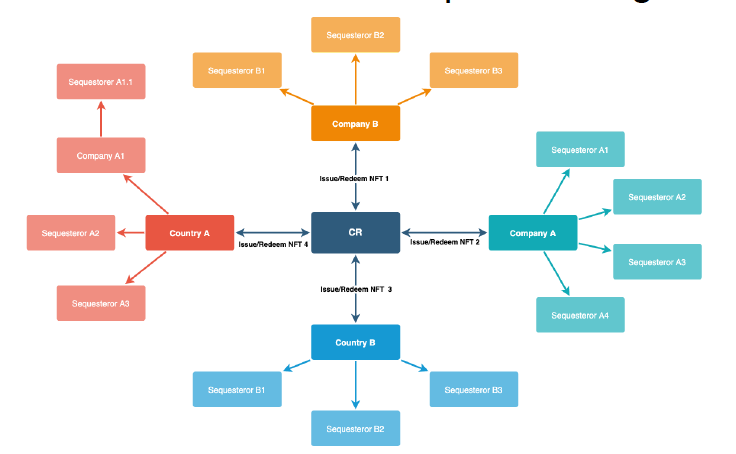
\includegraphics[width=4in]{red_green_issue.png}
\caption{Flow of NFT issuances and redemptions between pollution prevention stakeholders and sequesterors, which is all managed by CR and marks stakeholder relationship when burning Red tokens in exchange for Green} 
\label{fig:red_green_issue}
\end{figure} 

\subsection{Social Credit Component to UBI}

Using a carbon token incentive system would redistribute wealth, incentivize low carbon
technology and avoid the environmental taxes which hit the world’s poor the hardest.

In some systems the proposed UBI solutions are targeted to close the segregation between the rich and poor but come at the cost of political interference. However these systems rarely work in practice because of the lobbying from the wealthy which have power to unilaterally dismiss such systems that intend to close the gap through taxation on rich and profitable corporations (REF). Companies and people that move would ideally be met with similar taxation systems in other jurisdictions however we foresee these other jurisdictions may or may not comply depending on their own policies and mandates to grow local economies through immigration of these wealthy people and companies.

Using our carbon offset token program, governments can purchase carbon offsets, which are an efficient spend of budget against environmental impacts of its economy and reduce taxes to those that inhibit environmentally responsible spending habits (such as buying local and not going over their carbon footprint quota per person). Hence, creating a positive feedback loop to incentivize people to adapt their spending habits is a great way to find new efficiencies and invent \emph{greener} technologies due to increased demand for such technologies and services. The work here will be to assign carbon scores to goods and services and also assign spending against carbon ratings of goods and services. People that have a negative carbon footprint can be paid in Green tokens creating a powerful driver to reduce pollution and assigning monetary benefits which can be a social credit component to a UBI system, one which is tied to actual production and verified work.

\section{Proposed Design}

\subsection{Overview}

In the CR process, tokens move through a series of three states in an acyclic fashion. When the token is in a particular state, it can otherwise be defined as a Statetoken, and (as discussed in the previous section) can take on the characteristics of one of three forms (ie, Green, Red, and Black). Upon initial issuance, 100M Green tokens are issued by CR, and over time this supply is set to decrease, while the supply of Red and Black tokens rise from zero to some steady-state equilibrium over time. Fig \ref{fig:state_diagram} illustrates the state transition diagram where the nodes represent tokens and the arcs represent the direction and probability of a token transitioning to another over a unit of time.

\begin{figure}[h]
\centering
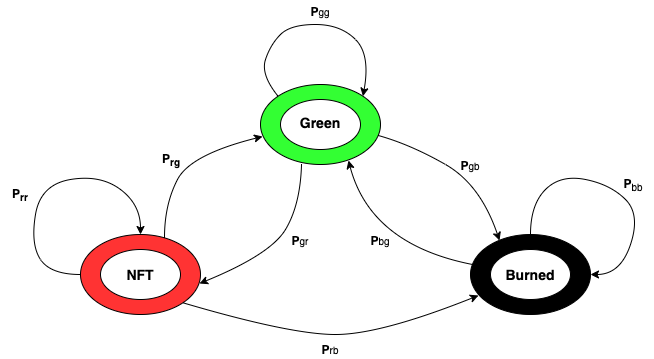
\includegraphics[width=4in]{state_diagram.png}
\caption{State transition diagram for Markov chain token model illustrating the probability of a token transitioning between states (ie, Green, NFT, and Burned) over a unit of time.} 
\label{fig:state_diagram}
\end{figure} 

Once the initial issuance of Green tokens has occurred, then pollution prevention stakeholders are issued one NFT asset for each partner, with assigned value based on their risk profile. The assigned value of the NFTs is denominated in Green tokens in the form of debt. This assigned value (denominated Green tokens) is based on the risk profile of the NFT holder (ie, akin to credit worthiness) which can be dynamically adjusted. These  pollution prevention stakeholders can assign tokens to various sequesters competing in various markets for those contract NFTs. Those NFTs, which have a unique value based on jurisdiction or cost, are sent to these sequesters and audited based on circumstances with those issuers and partner stakeholders.

The NFT stays in the possession of the sequesterer until the work has been performed and verified via the auditing process, see Fig \ref{fig:red_to_green}. Once complete, the NFT is burned and exchanged for both Black tokens as proof of sequestration and Green tokens which can be sold for revenue. Further to that, Black tokens can be held by sequesterer which when held over time slowly burn back into Green tokens. Each NFT may have its own rules, regulations and even sequestering costs factoring in base asset to NFT cost ratios.

\begin{figure}[h]
\centering
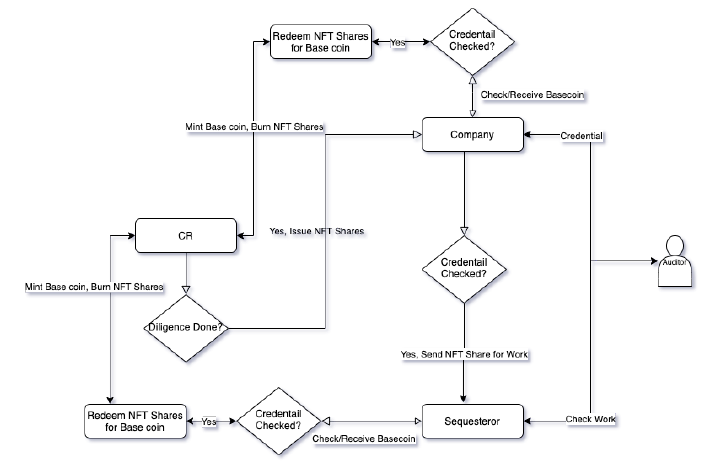
\includegraphics[width=4in]{red_to_green.png}
\caption{ Process workflow illustrating how Green tokens are minted through the auditing of Red NFT contracts } 
\label{fig:red_to_green}
\end{figure} 

Burning Green directly tokens can also result Black tokens directly by entering into the auditing process to apply credit to the pollution prevention stakeholder. Once Green tokens are burned the holder will receive Black tokens. Holding these tokens is advantageous over extended periods of time, which will result in the minting or new Green tokens. For instance, if the state transition probability from Black to Green is 0.01, then 100 Black tokens will produce 1 Green token and 99 Black tokens when the state transitions across one unit of time.

\begin{figure}[h]
\centering
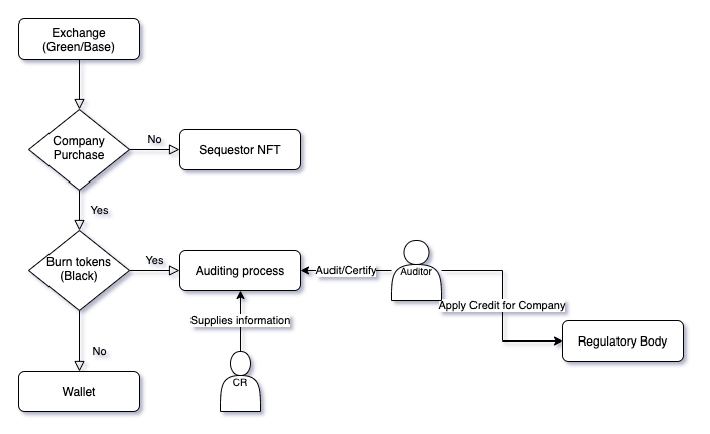
\includegraphics[width=4in]{green_to_black.png}
\caption{ Process workflow illustrating how Green tokens are burned to mint Black tokens } 
\label{fig:green_to_black}
\end{figure} 

Green token supply increases as sequestering happens and decreases as companies accumulate and burn Green tokens as proof that they have credits. If the rate of seqestration exceeds the rate of credit consumed by companies ,then the Green token supply is inflationary and is deflationary if sequestering doesn’t adequately satisfy the burning of credits to black. For the deflationaray case, sequestering services will naturally start to fill the demand and organically find equilibrium.


\subsection{Tokenized Company Shares}

It was requested that we create a fungible token for the purpose of share allocations in a company represented as a token product on blockchain. Also, these shares should not be transferable unless explicitly allowed by CR. We can enable this functionality on Syscoin through Notary services which will allow a case-by-case basis for transaction authorization between peer-to-peer (P2P) transfers. Here are the following token specifications:

Token to sell to raise funds
\begin{itemize}
\item \textbf{Max supply}: 100m
\item \textbf{Precision}: 8
\item \textbf{Total raise}: sell 10m upfront @ \$10
\item \textbf{Token symbol}: GCX
\end{itemize}

Token to issue as NFT for companies
\begin{itemize}
\item \textbf{Max supply}: MAX
\item \textbf{Precision}: 8
\item \textbf{Token symbol}: CX
\end{itemize}

Token received from burning GCX or CX
\begin{itemize}
\item \textbf{Max supply}: MAX
\item \textbf{Precision}: 8
\item \textbf{Token symbol}: BCX
\end{itemize}

Individual NFT:
\begin{itemize}
\item \textbf{Precision}: 8
\item \textbf{Max supply}: MAX
\end{itemize}

\subsection{Tokenomics}
\label{section:token_model}

Assume we are given the following stochastic (Markov) matrix:

\begin{equation*}
P = 
\begin{bmatrix}
p_{g,g} & p_{g,r}  & p_{g,b} \\
p_{r,g} & p_{r,r}  & p_{r,b} \\
p_{b,g} & p_{b,r} & p_{b,b} 
\end{bmatrix}
\end{equation*}

where each element is non-negative and each row sums to one. Each row of $P$ can be regarded as a probability mass function over $n$ possible outcomes. For instance, element $p_{g,b}$ represents the probability of a green token transitioning to a black token between states. For our problem, we setup the following transition matrix representing our business targets:

\begin{equation}
P_{\mu} = 
\begin{bmatrix}
0.95 & 0  & 0.05 \\
0.165 & 0.67  & 0.165 \\
0.01 & 0 & 0.99
\end{bmatrix}
\label{e:transition_matrix}
\end{equation}
where the frequency is monthly, and the states are represented as green, NFT, burned respectively. In Fig \ref{fig:state_diagram}, we represent this Markov process as a directed graph with edges labelled by the transition probabilities in (\ref{e:transition_matrix}).

Let's assume $\{X_{t}\}$ is a Markov chain with stochastic matrix $P$, and the distribution of $X_{t}$ to be $\psi_{t}$. Hence, if we let the initial distribution of $\psi_{0} = [1,0,0]$, the probability distribution of $X_{t}$ can be determined via:

\begin{equation}
X_{t} \sim \psi_{0}P^{t}
\label{e:pow_vs_pos}
\end{equation}

Hence, the estimated token supply at time $t$ is given by:
\begin{equation}
\hat{S}_{t} = (S_{0} + \alpha N_{t})\psi_{0}P^{t}
\label{e:token_supply}
\end{equation}
where $S_{0}$ is the initial token supply (ie, 100M Green, 0 NFT and 0 Black tokens), $N_{t}$ represents the NFT IOU rate, and $\alpha \in [0,1)$ represents the global quality factor (eg, 0.9).

\subsubsection{Token Model Simulation}

To simulate transition probabilities in $\mathbf{P}_{t}$, we use the Beta distribution:
\begin{equation}
\mathbf{p}_{m,n,t} \sim Beta(\alpha_{m,n},\beta_{m,n})
\end{equation}
where $m$ is the current state, $n$ is the previous state and $\beta_{m,n} = 1-\alpha_{m,n}$. The parameters $\alpha_{m,n}$ and $\beta_{m,n}$ are selected such that $E\{\mathbf{P}_{t}\}$ = $P_{\mu}$. It is important to keep in mind that this is a stationary model, hence the expected values are invariant to time. We ensure that the rows of the simulations of $\mathbf{P}_{t}$ sum to one by applying the following normalization:
\begin{equation}
P_{m,n,t}'= \dfrac{P_{m,n,t} }{  \sum_{n} P_{m,n,t}  }.
\end{equation}
where $P_{m,n,t}$ represents the an element of $\mathbf{P}_{t}$ at time $t$. The simulated token supply  at time $t$ is defined as:
\begin{equation}
\hat{\mathbf{S}}_{t} =(S_{0} + \alpha N_{t})\psi_{0}\mathbf{P}_{t}^{t}
\label{e:token_supply_simulation}
\end{equation}

\begin{table}[h!]
\centering
\begin{tabular}{|c c|c|c|c| } 
\hline
 & \multicolumn{4}{ c |}{ Next State } \\
 &  & Green & NFT & Burned \\
\hline
\multirow{ 3}{*}{Current State} & Green & $P(X_{n+1} = g | X_{n} = g )$ & $P(X_{n+1} = r | X_{n} = g )$ & $P(X_{n+1} = b | X_{n} = g )$ \\
& NFT & $P(X_{n+1} = g | X_{n} = r )$ & $P(X_{n+1} = r | X_{n} = r )$ & $P(X_{n+1} = b | X_{n} = r )$ \\
& Burned & $P(X_{n+1} = g | X_{n} = b )$ & $P(X_{n+1} = r | X_{n} = b )$ & $P(X_{n+1} = b | X_{n} = b )$ \\
\hline
\end{tabular}
\caption{Transition state matrix for token model detailing probabilities of transitioning from current to next state over a unit of time. The token states are denoted by Green $\rightarrow$ g, NFT $\rightarrow$ r, and Burred $\rightarrow$ b.}
\label{table:trans_state_matrix}
\end{table}

\begin{figure}
\centering
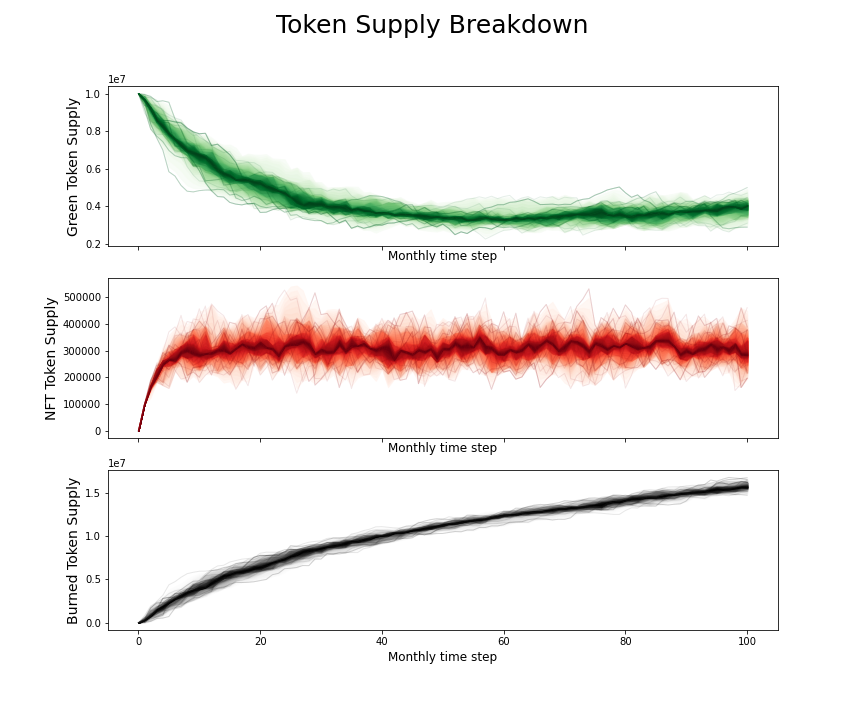
\includegraphics[width=4in]{token_supply_sims.png}
\caption{Markov Chain Token model simulations assuming stationary transition probabilities applying the Beta distribution at each time point at a monthly frequency. The expectations of the transition probability matrix (\ref{e:transition_matrix}) was selected based on business targets. The simulation begins with 100M Green tokens, the bulk of which will transition to red and black tokens over time and eventually reach a state of equilibrium. When the system reaches steady-state, the expected supply of each of the three tokens will remain constant.} 
\label{fig:token_supply_sims}
\end{figure} 

\begin{figure}
\centering
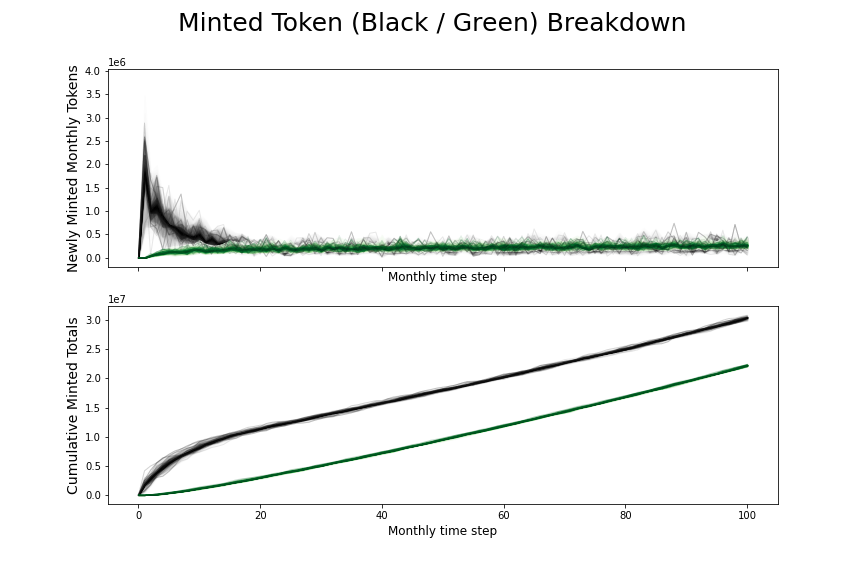
\includegraphics[width=4in]{burned_minted.png}
\caption{Newly minted green and burned tokens resulting from simulation model (\ref{e:token_supply_simulation}). Simulations of: (TOP) number of daily minted tokens; and (BOTTOM) cumulative number of daily minted tokens.} 
\label{fig:burned_minted}
\end{figure} 

\begin{figure}
\centering
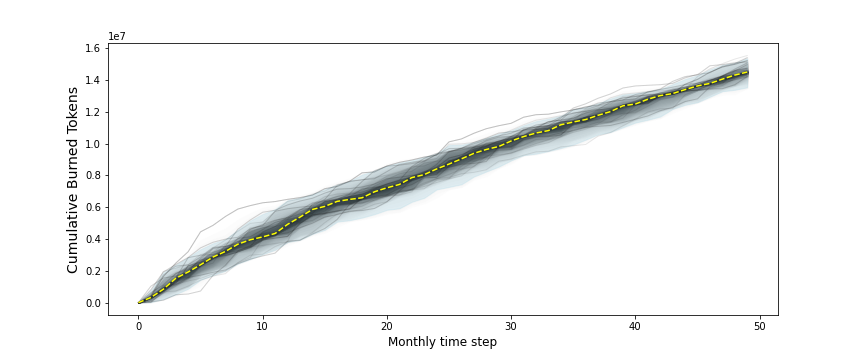
\includegraphics[width=4in]{burned_tokens.png}
\caption{Plot of simulated number of sequestered tons of carbon; this is determined bytaking the cumulative sum of Black tokens overtime } 
\label{fig:burned_tokens}
\end{figure} 

\subsection{Revenue Model}

Both Green and Black tokens are fungible hence tradable on exchanges, but serve different ways to generate revenue. Green tokens are earned from sequestoring carbon (ie, through NFT to Green token conversions) which can be sold for profit. Black tokens are earned through burning NFT or Green tokens. These Black tokens can be held privately which burn slowly over time (ie, at a pre-determined rate set by CR) producing Green tokens that can sold for profit or utilized back into the system. Aside from the tokens themselves, value added services such as softwares, wallets are other revenue generating options that companies may pay services for.

\begin{table}[h]
\centering
\begin{tabular}{ |c|c|c|c| } 
\hline
 Year & median & lwr 5\% & upr 95\% \\
\hline
1 & 4,730,000 & 3,080,000 & 6,230,000 \\
2 & 7,960,000 & 7,040,000 & 9,690,000 \\
3 & 11,000,000 & 9,800,000 & 12,260,000 \\
4 & 13,620,000 & 12,100,000 & 14,770,000  \\
5 & 16,060,000 & 15,120,000 & 19,710,000 \\
\hline
\end{tabular}
\caption{Simulated number of sequestered tons of Carbon assuming transition matrix (\ref{table:revenue_model}) as business targets}
\label{table:pow_vs_pos}
\end{table}


\section{Management on Jurisdictional Level}

From time to time, companies may need cooperation with local governments who have requirements to fulfill quotas for its jurisdiction, which can be managed using a number of strategies. First, companies can buy directly from a local sequestration provider, and buy their NFT’s for a premium (ie, move to front of queue) which can been converted to Green tokens from CR (ie, pay requisite small fees for doing so). Upon fulfilling the needs of the NFT contract, tokens are then burned as described in Section \ref{section:nft_tokens}. Contracts would be directly created between NFT partners and sequestration companies, hence localized based on jurisdiction. Alternatively, companies can skip the auditing process and buy directly from CR via the aforementioned queue. Doing this puts more demand on those jurisdictions to produce more sequestration and would be an option if enough sequestration services are available. Finally, premiums paid for these higher demands are not factored into the Green token market unless larger market players drive prices upwards as global aggregate prices go up.

Evidence of the sequestration audit trail would need to be timestamped and recorded on the blockchain, which would be publicly accessible through a provided hyperlink in the asset public data field. This would be a live document that would update with signatures of auditors registered with Digital Identities and along with any associated metadata. The timestamped log will bring about transparency between consumed sequestrations, the actual registered audited sequestrations and allow one to audit that the supply of Basecoin’s accurately represents the audited sequestration amounts since one token can represent a certain amount of Carbon sequestration tonnage. It will allow companies to know what is available for consumption should there be requirements around jurisdictional consumption.

If companies require localized sequestration in exchange for burning Green tokens, then CR can select which sequestorers will qualify for which particular carbon credit application. Upon completion, tokens are burned and the time stamped audit trail is updated to reflect \emph{consumed} sequestrations. For instance, say MSFT requires 100 tons of American sequestration, and we have 100 tons of American sequestration in the audit trail, we can then choose those sequestrations and label them as consumed. Future American sequestration requests either need to pay the American sequestors, or wait for more sequestrations to register from American sequestors. However, under normal circumstances, the audit trail can be processed sequentially.

It would be ideal to manage such an effort at the global level (eg, under L'Accord de Paris) so that there are no jurisdictional requirements. Otherwise, the incentive would be to negotiate with companies directly. If the sequestration is fungible, the system can be more effectively managed through better supply stabilization and demand dynamics. For instance, this can be analogous to the Euro currency, where multiple countries, each with their own policies, utilize a single currency. This may be less ideal, but having this managed under a single policy may help avoid chances of corruption. However, we may not have control over this, and so we can employ this strategy upon further investigation, if need be.

\subsection{Competition}

There are number of similar blockchain-based carbon crediting  projects that are currently underway globally. As far as tradable Carbon credit tokens go, we have AirCarbon \cite{AirCarbon}, Carbonx \cite{Carbonx} and Verra. Each of these platforms focus on securitizing carbon credits with slight differences in how this service will be delivered like what we are proposing with CR. However, projects like SolarCoin \cite{SolarCoin} and Nori \cite{Nori} have more of a niche market. For instance, SolarCoin provide incentives to invest in solar installations which when monetized over time becomes effectively free.  Whereas the Verra program catalyzes measurable climate action and sustainable development outcomes by enticing large-scale investment to activities to reducing emissions.

When it comes to securitizing carbon credits, CR is unique as it leverages the technological advantages that NFT provides so that pollution prevention companies and sequestration service providers can create contracts customized to the  stakeholders needs in accordance to the jurisdiction which they fall under.

\subsection{Cost of CO$_{2}$ Capture and Storage}

There have been a number of studies and whitepapers addressing methodological tools and surveys to help discover the cost of carbon sequestration \cite{Mck09,Gil18,Mck21,Sch20,Dav00,Rub15,Rub07}. To establish a global market for the cost of carbon would require some background understanding of the cost of CO$_{2}$, capture and storage (CCS) process. According to \cite{Rub15}, this can be sub-divided into two main purposes: (a) technology assessments to support things like capital investments and  technology selection; and (b) policy assessments to support things like legislative and regulatory issues. Methodologies into the determination of these carbon costs using a host technical and economic assumptions as well as tabulated calculations have been well covered in \cite{Dav00,Rub07,Rub15}.

Marginal cost is a concept applied in economics that measures the cost of implementing addition units into a system. Whereas abatement cost is defined as the cost of reducing things that negatively impact the environment. Marginal abatement cost is the cost of reducing one unit of pollution, usually measured in metric tons of CO$_{2}$. A well-known tool for monitoring theses costs is the marginal abatement cost curve, which is a widely used tool that was popularized by well-known organizations like Mckinsey through the utilization of their Greenhouse gas (GHG) abatement curve \cite{Mck09}. It is through the use of such tools that researchers and policy makers can collaborate to begin to first necessary steps of price discovery consolidated into a tradable global carbon market. 

Regarding actual costs, a research study for the region northeastern and midwestern United States  suggests coal-sourced CO$_{2}$ emissions can be stored at a cost of \$52–\$60 tonne, whereas the cost to store emission from natural-gas-fired plants ranges from approximately \$80 to \$90 \cite{Sch20}. A Harvard study has found fossil fuel power plants with carbon capture and storage costs estimated cost of \$43 to \$95 US per tonne \cite{Gil18}. In Canada, the current level of carbon tax is approximately \$30 per tonne (see Figure \ref{figure:nation_carbon_taxes}), and is anticipated to top out at \$50 per tonne in 2022. According to Canada's Healthy Environment and Healthy Economy (HEHE) plan, that figure is scheduled to rise to \$170 per tonne incrementally until the year 2030 \cite{Mck21}. By referring to available data on national carbon tax prices for 2021 from the World Bank in Fig. \ref{figure:nation_carbon_taxes}, the median of \~ \$28 per tonne (REF).



\begin{figure}[h]
\centering
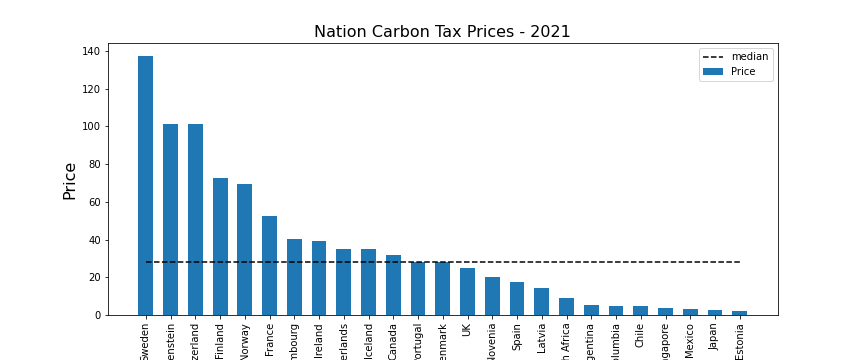
\includegraphics[width=5in]{nation_carbon_taxes.png}
\caption{National carbon tax prices for 2021; source can be found in \cite{WBank}. We can see large  between the various jurisdictions, and provides some insight as to which jurisdiction that may offer the best operating costs. This is akin to the variations in cost of electricity for various regions which serves as the base cost for Bitcoin's PoW .} 
\label{figure:nation_carbon_taxes}
\end{figure} 

\subsection{Carbon Exchange Rate: Speculative vs Stable}

Regarding the Green token to Carbon exchange rate, we adopt a hybrid model. That is offering both a fixed and floating speculative rate to users of the system. This is done by allowing a floating speculative rate for companies requiring credits (ie, Green Tokens), while at the same time allowing for the setting of stable rates through the offloading of speculative risks for companies dealing with sequestering. Doing this allows for more responsive supply side mechanics of Green tokens (ie, carbon credits).

Regarding the stable component we keep the ratio as a constant 1:1; that is one Green token for one one ton of sequestered Carbon. Doing this removes the need for governments and large enterprises to have to make speculative purchases, hence make the system more usable. The number of new minted tokens depends on the number of new tons of carbon that are being introduced into the atmosphere. If the amount of new Carbon being sequestered globally is greater than new pollution then Green tokens become deflationary, otherwise it's inflationary.

Alternatively, regarding the speculative component, we begin the process with a 1:1 ratio, however the ratio changes as tokens are burned over time. Hence, making one ton of carbon to be less than one Green token. This model adds speculation enticing enterprises to purchase and remove tokens from the supply which reduce costs over time and also for potential gains. While the dollars cost value remains consistent, the number of tokens required for one ton of carbon emissions drops. Hence putting deflationary pressures on the supply.

\section{Summary}

In this whitepaper we propose a Carbon offset design program using blockchain Tokenization. The advantages to using such technology are: (a) minimizes red tape allowing for improved accessibility; (b) improves efficiency by allowing for direct peer-to-peer transactions eliminating third part involvement; (c) provides transparency and trust on an immutable public ledger database; (d) provides global access across various jurisdictions; and (e) drives new payment innovations that go beyond the limitations of current fiat money system. Our proposal is comprised of three tokens (Green, Red, and Black tokens); the action of transitioning from one token state to another is called burning. Green tokens are required to enter into the Carbon offsetting process directly and are awarded as work done via the auditing process. Next, NFT tokens serve as IOU contracts to sequester Carbon. Finally, Black tokens serve as proof of burn which can be staked to gain more Green tokens as incentives.  

\section{To-dos: Research, Analysis and Presentation}

\begin{itemize}
\item Some education background on the Carbon sequestration process (literature review)
\item Carbon sequestration work/costs is akin to electricity costs and different jurisdictions will have different sequestration costs
\item \$10 per token to 1 ton of Carbon: needs research to determine costs
\item Carbon sequestration is subjective and no trust-less  as whole thing can be corrupted by few auditors
\begin{itemize}
\item need to think about concessions to be put in place to thwart these potential bad actors
\end{itemize}
\item Creating a standards body to work with stakefish/f2pool and other miners to find a way to
specify how carbon offsets can be applied to the industry effectively
\item Understand Automated Market Maker (AMM) model pertaining to a more distributed system where sequestorers can be direct to market
\item Potential market avenues (ie, Bitcoin miners )
\item Come up with plan for potential simulation or some other quantitative analysis around carbon exchange rate
\item Re-work existing presentation
\item Missing: software architecture of the token project
\end{itemize}


\label{section:summary}

\begin{thebibliography}{1}


\bibitem{Kal96} E. Kalnay et. al., \textit{The NCEP/NCAR 40-Year Reanalysis Project}, Bulletin of the American Meteorological Society, 1996, pp. 77437-471

\bibitem{Ten00} J.B. Tenenbaum, V. Silva and J.C. Langford, \textit{A Global Geometric Framework for Nonlinear Dimensionality. Reduction}. Science, v. 290 no.5500, 2000.

\bibitem{Hij05} R.J. Hijmans, S.E. Cameron, J.L. Parra, P.G. Jones, A. and Jarvis, \textit{Very High Resolution Interpolated Climate Surfaces for Global Land Areas}, International Journal of Climatology, Vol. 25, 2005

\bibitem{Ali21} Ian Alison, \textit{Blockchain Coalition Launches Tradable Carbon Credit Token}, Accessed on: Jul 2021. [Online]. https://www.coindesk.com/blockchain-coalition-launches-tradable-carbon-credit-token

\bibitem{Syscoin} \textit{Syscoin: Network-enforced Business Rulesets}, Accessed on: Jul 2021. [Online]. https://github.com/syscoin/sips/blob/master/sip-0002.mediawiki

\bibitem{SolarCoin} \textit{SolarCoin is a cryptocurrency that incentivizes a solar-powered planet}, Accessed on: Jul 2021. [Online]. https://solarcoin.org/

\bibitem{AirCarbon} \textit{A digital exchange focused on eliminating market friction in a carbon constrained economy.}, Accessed on: Jul 2021. [Online]. https://www.aircarbon.co/

\bibitem{Carbonx} \textit{A Personal Carbon Trading Inc.}, Accessed on: Jul 2021. [Online]. hhttps://www.carbonx.ca/

\bibitem{Nori} \textit{The Nori Carbon Removal Marketplace}, Accessed on: Jul 2021. [Online]. https://nori.com/

\bibitem{Microsoft21} \textit{Microsoft Bought Carbon Credits Through Cosmos Blockchain}, Accessed on: Jul 2021. [Online]. https://thecoinshark.net/blockchain-news/microsoft-bought-carbon-credits-through-cosmos-blockchain

\bibitem{Pan19} Y. Pan, X. Zhanga, Y. Wanga, J. Yan, S. Zhou, G. Li, J. Bao, \textit{Application of Blockchain in Carbon Trading}, \emph{Energy Procedia}., vol. 1588, no. 7, Feb. 2019.

\bibitem{NET19} National Academies of Sciences, Engineering, and Medicine, \textit{Negative Emissions Technologies and Reliable Sequestration: A Research Agenda (2019)}, The National Academies Press, Washington, DC, 2019 

\bibitem{Mic21}  \textit{Microsoft carbon removal: Lessons from an early corporate purchase}, Accessed on: Jul 2021. [Online]. https://www.microsoft.com/en-us/corporate-responsibility/sustainability/carbon-removal-program

\bibitem{Glo21} \textit{Global Warming of 1.5 ºC}, Accessed on: Jul 2021. [Online]. https://www.ipcc.ch/sr15/

\bibitem{DOE16} \textit{Carbon Capture, Utilization, and Storage: Climate Change, Economic Competitiveness, and Energy Security}, US Department of Energy, 2016, Accessed on: Jul 2021. [Online]. https://www.energy.gov/fe/downloads/doe-white-paper-carbon-capture-utilization-and-storage

\bibitem{Cri20} M. Crippa, D. Guizzardi, M. Muntean, and E. Schaaf, \textit{Fossil CO2 emissions of all world countries - 2020 Report}, Publications Office of the European Union, Luxembourg, Sept 2020.

\bibitem{Liu20} Z. Liu et al.,  \textit{Global energy review: CO2 emissions in 2020}, Dec 2021. Accessed on: Dec 2020 [Online]. Available: https://arxiv.org/abs/2012.00854

\bibitem{CDCS05} \textit{Carbon Dioxide Capture and Storage}, Intergovernmental Panel on Climate Change, Cambridge University Press, 2005.

\bibitem{EDGAR19} \textit{European Commission, Joint Research Centre (EC-JRC)/Netherlands Environmental Assessment Agency (PBL)}. Emissions Database for Global Atmospheric Research (EDGAR), release EDGAR v5.0 (1970 - 2015) of November 2019.

\bibitem{Mck09} McKinsey \& Company, \textit{Impact of the Financial Crisis on Carbon Economics: Version 2.1 of the Global Greenhouse Gas Abatement Cost Curve}, 2009. 

\bibitem{Gil18} K. Gillingham and J. H. Stock \textit{The Cost of Reducing Greenhouse Gas Emissions} Journal of Economic Perspectives—Vol. 32, No. 4, Fall 2018, pp. 53–72

\bibitem{Sch20} W. Schmelz, G. Hochman, K. Miller, \textit{Total cost of carbon capture and storage implemented at a regional scale: northeastern and midwestern United States}. In Interface Focus. 10 (5), p. 20190065, 2020

\bibitem{Dav00} J. David, H.J. Herzog, \textit{The cost of carbon capture}, Fifth International Conference on Greenhouse Gas Control Technologies (GHGT-5), Cairns, Australia, Aug 13–16, 2000.

\bibitem{Rub15} E. Rubin, J. David and  H.J. Herzog, \textit{The cost of CO2 capture and storage}, International Journal of Greenhouse Gas Control, Vol. 40, Sept. 2015, pp 378-400

\bibitem{Rub07} E. Rubin, C. Chen and A. Rao, \textit{Cost and performance of fossil fuel power plants with CO2 capture and storage}, Energy Policy, Vol. 35, Issue 9, Sept. 2007, Pages 4444-4454

\bibitem{CBC19} E. Chung, \textit{Carbon capture: What you need to know about catching CO2 to fight climate change}, CBC Science, Sep 2019, Accessed on: Jul 2021. [Online]. https://www.cbc.ca/news/science/carbon-capture-faq-1.5250140

\bibitem{WBank} \textit{Worldbank Carbon Pricing Dashboard}, Accessed on: Jul 2021. [Online]. https://carbonpricingdashboard.worldbank.org/map\_data

\bibitem{Mck21} R. McKitrick and E. Aliakbari, Estimated Impacts of a \$170 Carbon Tax in Canada, Fraser Institute, 2021

\end{thebibliography}



\end{document}
